\chapter{Appendix}
\clearpage

\section{Declaration of Authorship} \label{Declaration of Authorship}
We hereby certify that the thesis we are submitting is entirely our own original work except where otherwise indicated.
We are aware of the University's regulations concerning plagiarism, including those regulations concerning disciplinary actions that may result from plagiarism.
Any use of the works of any other author, in any form, is properly acknowledged at their point of use.
Furthermore, we would like to disclose that we have utilized the assistance of ChatGPT, an artificial intelligence language model developed by OpenAI,
to improve the clarity and coherence of the text. While ChatGPT has provided suggestions and refinements,
the overall content, ideas and analysis presented in this thesis remain our own.

\bigskip
\textbf{Location, Date} \\
Rapperswil, 24. January 2024

\vspace{1.2cm}
\begin{tabular}{@{}p{0.1cm}p{6cm}p{0.6cm}p{6cm}@{}}
	 & \hrulefill          &  & \hrulefill   \\ \\[-0.7em]
	 & Florian Baumgartner &  & Alain Keller \\
\end{tabular}


\includegraphics[width=4.8cm, align=t, smash=br, hshift=0.9cm, vshift=2.55cm]{appendix/Signature_Florian_Baumgartner.pdf}
% \includegraphics[width=3.6cm, align=t, smash=br, hshift=8.25cm, vshift=2.2cm]{appendix/Signature_Alain_Keller.pdf}
\todo{Add Alain's signature here}
\newpage

\section{Data Archive} \label{Data Archive}
All created files and documents of this project are publicly available on GitHub. An institution called \textbf{PA-OST-2023} (\url{https://github.com/PA-OST-2023}) has been founded which contains repositories for each individual part of the project.
A quick description of the repositories including the associated web link is listed below:

\subsubsection{heron-administration} \vspace{-0.2cm}
\begin{description}
	\item[Description:] This repository contains all confidential information of the project.\vspace{-0.25cm}
	\item[URL:] \url{https://github.com/PA-OST-2023/heron-administration}\vspace{-0.25cm}
	\item[Type:] Private\vspace{-0.25cm}
\end{description}

\subsubsection{heron-literature} \vspace{-0.2cm}
\begin{description}
	\item[Description:] This repository contains all literature used in this project.\vspace{-0.25cm}
	\item[URL:] \url{https://github.com/PA-OST-2023/heron-literature}\vspace{-0.25cm}
	\item[Type:] Private\vspace{-0.25cm}
\end{description}

\subsubsection{heron-documentation} \vspace{-0.2cm}
\begin{description}
	\hfuzz=35.0pt
	\item[Description:] This repository contains this document.\vspace{-0.25cm}
	\item[URL:] \url{https://github.com/PA-OST-2023/heron-documentation}\vspace{-0.25cm}
	\item[Type:] Public\vspace{-0.25cm}
\end{description}

\subsubsection{heron-hardware} \vspace{-0.2cm}
\begin{description}
	\item[Description:] This repository contains hardware related documents (Schematics, PCB).\vspace{-0.25cm}
	\item[URL:] \url{https://github.com/PA-OST-2023/heron-hardware}\vspace{-0.25cm}
	\item[Type:] Public\vspace{-0.25cm}
\end{description}

\subsubsection{heron-firmware} \vspace{-0.2cm}
\begin{description}
	\item[Description:] This repository contains firmware source code written in C++.\vspace{-0.25cm}
	\item[URL:] \url{https://github.com/PA-OST-2023/heron-firmware}\vspace{-0.25cm}
	\item[Type:] Public\vspace{-0.25cm}
\end{description}

\subsubsection{heron-simulator} \vspace{-0.2cm}
\begin{description}
	\item[Description:] This repository contains the simulator source code written in Python.\vspace{-0.25cm}
	\item[URL:] \url{https://github.com/PA-OST-2023/heron-simulator}\vspace{-0.25cm}
	\item[Type:] Public\vspace{-0.25cm}
\end{description}

\subsubsection{heron-application} \vspace{-0.2cm}
\begin{description}
	\item[Description:] This repository contains the application source code written in Python.\vspace{-0.25cm}
	\item[URL:] \url{https://github.com/PA-OST-2023/heron-application}\vspace{-0.25cm}
	\item[Type:] Public\vspace{-0.25cm}
\end{description}

\subsubsection{heron-mechanical} \vspace{-0.2cm}
\begin{description}
	\item[Description:] This repository contains mechanical related documents (CAD-Files).\vspace{-0.25cm}
	\item[URL:] \url{https://github.com/PA-OST-2023/heron-mechanical}\vspace{-0.25cm}
	\item[Type:] Public\vspace{-0.25cm}
\end{description}

\subsubsection{heron-bastelstube} \vspace{-0.2cm}
\begin{description}
	\item[Description:] This repository contains temporary and experimental files.\vspace{-0.25cm}
	\item[URL:] \url{https://github.com/PA-OST-2023/heron-bastelstube}\vspace{-0.25cm}
	\item[Type:] Private\vspace{-0.25cm}
\end{description}
\newpage

\section{Definition of Task} \label{definition_of_task}
\enlargethispage{2.5cm}
\begin{adjustwidth}{0.23cm}{0cm} \hfuzz=7.0pt \vfuzz=19.0pt
	\makebox[\textwidth]{\frame{
\includegraphics[width=17.3cm, page=1]{appendix/Project_Definition_Audio_Localization.pdf}}}
\end{adjustwidth}
\newpage

\begin{adjustwidth}{-0.23cm}{0cm} \hfuzz=7.0pt \vfuzz=19.0pt
	\makebox[\textwidth]{\frame{
\includegraphics[width=17.3cm, page=2]{appendix/Project_Definition_Audio_Localization.pdf}}}
\end{adjustwidth}
\newpage

\section{Datasheet of MEMS Microphone (MP34DT05TR-A)} \label{appendix_datasheet_microphone}
\enlargethispage{2.5cm}
\begin{adjustwidth}{0.23cm}{0cm} \hfuzz=7.0pt \vfuzz=19.0pt
	\makebox[\textwidth]{\frame{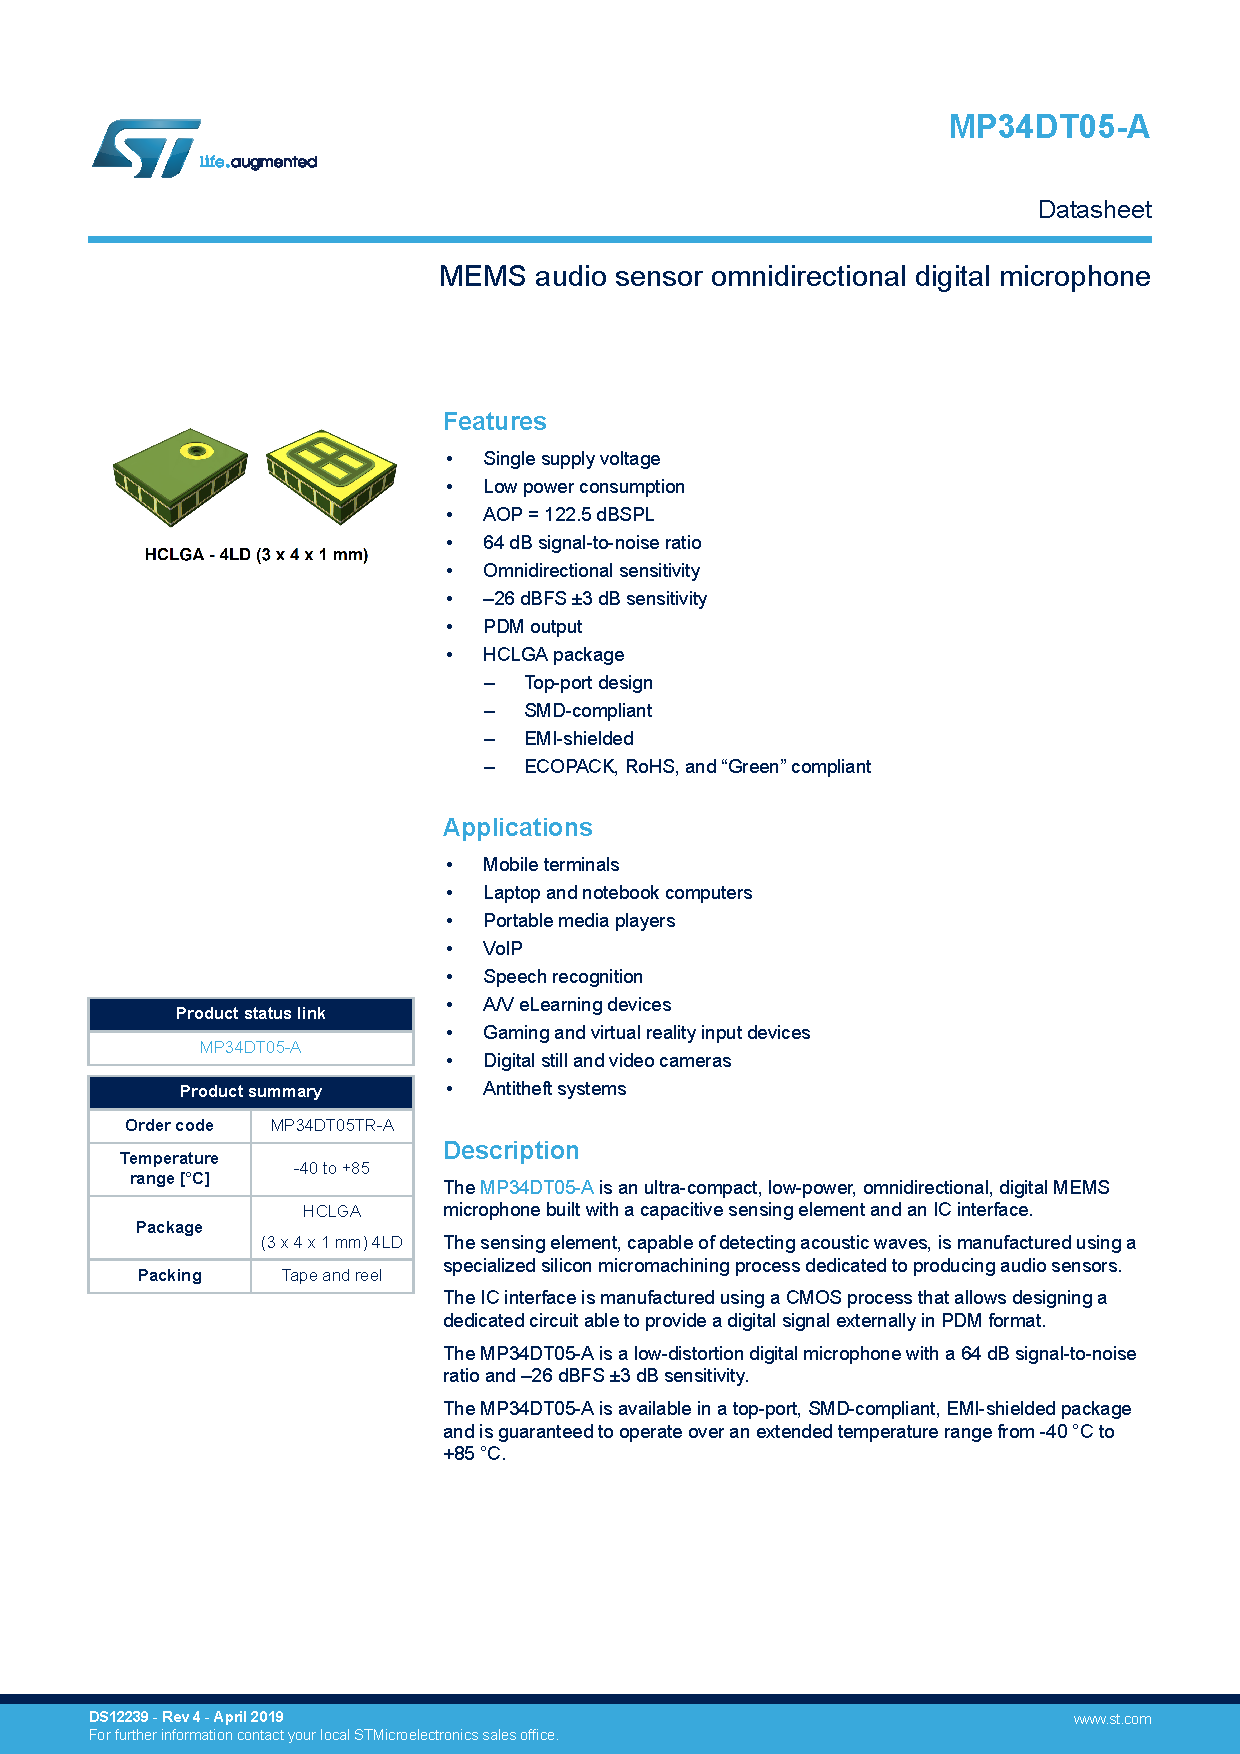
\includegraphics[angle=0, width=17.3cm, page=1]{appendix/Microphone_Datasheet.pdf}}}
\end{adjustwidth}
\newpage


% \section{Audio-Beamformer Schematics} \label{Fleet-Monitor V1.0 Schematics}
% \enlargethispage{2.5cm}
% \begin{adjustwidth}{0.23cm}{0cm} \hfuzz=7.0pt \vfuzz=20.0pt
% \makebox[\textwidth]{\includegraphics[angle=90, width=17.3cm, page=1]{appendix/Audio-Beamformer.pdf}}
% \end{adjustwidth}
% \newpage

% \begin{adjustwidth}{-0.23cm}{0cm} \hfuzz=7.0pt \vfuzz=20.0pt
% \makebox[\textwidth]{\includegraphics[angle=90, width=17.3cm, page=2]{appendix/Audio-Beamformer.pdf}}
% \end{adjustwidth}
% \newpage

% \begin{adjustwidth}{0.23cm}{0cm} \hfuzz=7.0pt \vfuzz=20.0pt
% \makebox[\textwidth]{\includegraphics[angle=90, width=17.3cm, page=3]{appendix/Audio-Beamformer.pdf}}
% \end{adjustwidth}
% \newpage

% \begin{adjustwidth}{-0.23cm}{0cm} \hfuzz=7.0pt \vfuzz=20.0pt
% \makebox[\textwidth]{\includegraphics[angle=90, width=17.3cm, page=4]{appendix/Audio-Beamformer.pdf}}
% \end{adjustwidth}
% \newpage

% \begin{adjustwidth}{0.23cm}{0cm} \hfuzz=7.0pt \vfuzz=20.0pt
% \makebox[\textwidth]{\includegraphics[angle=90, width=17.3cm, page=5]{appendix/Audio-Beamformer.pdf}}
% \end{adjustwidth}
% \newpage

% \begin{adjustwidth}{-0.23cm}{0cm} \hfuzz=7.0pt \vfuzz=20.0pt
% \makebox[\textwidth]{\includegraphics[angle=90, width=17.3cm, page=6]{appendix/Audio-Beamformer.pdf}}
% \end{adjustwidth}
% \newpage

% \begin{adjustwidth}{0.23cm}{0cm} \hfuzz=7.0pt \vfuzz=20.0pt
% \makebox[\textwidth]{\includegraphics[angle=90, width=17.3cm, page=7]{appendix/Audio-Beamformer.pdf}}
% \end{adjustwidth}
% \newpage

% \begin{adjustwidth}{-0.23cm}{0cm} \hfuzz=7.0pt \vfuzz=20.0pt
% \makebox[\textwidth]{\includegraphics[angle=90, width=17.3cm, page=8]{appendix/Audio-Beamformer.pdf}}
% \end{adjustwidth}
% \newpage

% \begin{adjustwidth}{0.23cm}{0cm} \hfuzz=7.0pt \vfuzz=20.0pt
% \makebox[\textwidth]{\includegraphics[angle=90, width=17.3cm, page=9]{appendix/Audio-Beamformer.pdf}}
% \end{adjustwidth}
% \newpage

% \begin{adjustwidth}{-0.23cm}{0cm} \hfuzz=7.0pt \vfuzz=20.0pt
% \makebox[\textwidth]{\includegraphics[angle=90, width=17.3cm, page=10]{appendix/Audio-Beamformer.pdf}}
% \end{adjustwidth}
% \newpage

% \section{PCB Top-Layer}
% \enlargethispage{2.5cm}
% \begin{adjustwidth}{0.23cm}{0cm} \hfuzz=7.0pt \vfuzz=19.0pt
% \makebox[\textwidth]{\frame{\includegraphics[width=17.3cm, trim=75mm 12mm 67mm 6mm, clip, page=11]{appendix/Audio-Beamformer.pdf}}}
% \end{adjustwidth}
% \newpage

% \section{PCB Bottom-Layer}
% \enlargethispage{2.5cm}
% \begin{adjustwidth}{-0.23cm}{0cm} \hfuzz=7.0pt \vfuzz=19.0pt
% \makebox[\textwidth]{\frame{\includegraphics[width=17.3cm, trim=67mm 12mm 75mm 6mm, clip, page=12]{appendix/Audio-Beamformer.pdf}}}
% \end{adjustwidth}
% \newpage

% \section{PCB Top-Overlay}
% \enlargethispage{2.5cm}
% \begin{adjustwidth}{0.23cm}{0cm} \hfuzz=7.0pt \vfuzz=19.0pt
% \makebox[\textwidth]{\frame{\includegraphics[width=17.3cm, trim=75mm 12mm 67mm 6mm, clip, page=13]{appendix/Audio-Beamformer.pdf}}}
% \end{adjustwidth}
% \newpage

% \section{PCB Bottom-Overlay}
% \enlargethispage{2.5cm}
% \begin{adjustwidth}{-0.23cm}{0cm} \hfuzz=7.0pt \vfuzz=19.0pt
% \makebox[\textwidth]{\frame{\includegraphics[width=17.3cm, trim=67mm 9mm 75mm 6mm, clip, page=14]{appendix/Audio-Beamformer.pdf}}}
% \end{adjustwidth}
% \newpage

% \section{PCB Outline}
% \enlargethispage{2.5cm}
% \begin{adjustwidth}{0.23cm}{0cm} \hfuzz=7.0pt \vfuzz=19.0pt
% \makebox[\textwidth]{\frame{\includegraphics[width=17.3cm, trim=65.5mm 1mm 67mm 0mm, clip, page=15]{appendix/Audio-Beamformer.pdf}}}
% \end{adjustwidth}
% \newpage


% \section{Bill of Materials (BOM)}
% \enlargethispage{2.5cm}
% \begin{adjustwidth}{-0.23cm}{0cm} \hfuzz=7.0pt \vfuzz=20.0pt
% \makebox[\textwidth]{\includegraphics[width=17.3cm, trim=45mm 104mm 64mm 76mm, clip]{appendix/Audio-Beamformer BOM.pdf}}
% \end{adjustwidth}
% \newpage


% \section{Mechanical Drawing Top-Plate}
% \enlargethispage{2.5cm}
% \begin{adjustwidth}{0.23cm}{0cm} \hfuzz=7.0pt \vfuzz=20.0pt
% \makebox[\textwidth]{\includegraphics[angle=90, width=17.3cm]{appendix/Topplate.pdf}}
% \end{adjustwidth}
% \newpage

% \section{Mechanical Drawing Base-Plate}
% \enlargethispage{2.5cm}
% \begin{adjustwidth}{-0.23cm}{0cm} \hfuzz=7.0pt \vfuzz=20.0pt
% \makebox[\textwidth]{\includegraphics[angle=90, width=17.3cm]{appendix/Baseplate.pdf}}
% \end{adjustwidth}
% \newpage

% \section{Mechanical Drawing Connecting-Bar}
% \enlargethispage{2.5cm}
% \begin{adjustwidth}{0.23cm}{0cm} \hfuzz=7.0pt \vfuzz=20.0pt
% \makebox[\textwidth]{\includegraphics[angle=90, width=17.3cm]{appendix/Connecting-Bar.pdf}}
% \end{adjustwidth}
% \newpage


% Schematics of Microphone Boards
% PCB Design of Microphone Boards
% BOM of Microphone Boards
% Schematics of Acquisition-System
% PCB Design of Acquisition-System
% BOM of Acquisition-System
% Schematics of Mainboard
% PCB Design of Mainboard
% BOM of Mainboard
% Schematics of Microphone-Arms
% PCB Design of Microphone-Arms
% BOM of Microphone-Arms
% Schematics of Angle-Sensor
% PCB Design of Angle-Sensor
% BOM of Angle-Sensor
% Mechanical Drawings of each component
